%% START OF FILE main.tex

%% ====================================================================
%% DOCUMENT CLASS AND PACKAGES
%% ====================================================================
%% The first command in your LaTeX source must be the \documentclass command.
\documentclass{ceurart}

%% One can fix some overfulls
\sloppy

%% Minted listings support 
%% Need pygment <http://pygments.org/> <http://pypi.python.org/pypi/Pygments>
\usepackage{listings}
%% auto break lines
\lstset{breaklines=true}

%% Document-specific packages from the original manuscript
% \usepackage{lmodern}
% \emergencystretch=3em
% \microtypesetup{expansion=false}

\usepackage{booktabs}
\usepackage{tabularx}
\usepackage{array}
\usepackage{makecell}
\usepackage{adjustbox}
\usepackage{algorithm}
\usepackage{enumitem}
\usepackage{amsmath,amssymb}
\usepackage{graphicx}
\usepackage{tikz}
\usetikzlibrary{arrows.meta,positioning,shapes.geometric}
\graphicspath{{figures/}}

%% Custom environments and commands
% \newcounter{algorithm}
% \newenvironment{algorithmblock}[1]{%
%   \refstepcounter{algorithm}\par\medskip
%   \noindent\begin{minipage}{\linewidth}\hrule\smallskip
%   \textbf{Algorithm \thealgorithm: #1}\par\smallskip\small
% }{%
%   \smallskip\hrule\end{minipage}\par\medskip
% }

\newcommand{\matA}{\mathbf{A}}
\newcommand{\matB}{\mathbf{B}}
\newcommand{\hatB}{\widehat{\mathbf{B}}}
\newcommand{\matT}{\mathbf{T}}
\newcommand{\matS}{\mathbf{S}}
\newcommand{\Rule}{\mathcal{R}}
\newcommand{\Dset}{\mathcal{D}}
\newcommand{\R}{\mathbb{R}}
\newcommand{\MMS}{M\&Ms}
\DeclareMathOperator*{\argmin}{arg\,min}
\DeclareMathOperator*{\argmax}{arg\,max}
\hypersetup{hypertexnames=false}

%% ====================================================================
%% MAIN DOCUMENT
%% ====================================================================
\begin{document}

%% ====================================================================
%% METADATA AND TITLE
%% ====================================================================
%% Rights management information.
\copyrightyear{2026}
\copyrightclause{Copyright for this paper by its authors. Use permitted under Creative Commons License Attribution 4.0 International (CC BY 4.0).}

%% This command is for the conference information
\conference{ICST-ODESA: International Scientific and Practical Conference ``Information Control Systems and Technologies'', September, 22--24, 2026}

%% The "title" command
\title{Auditing Deep Learning for Cardiac MRI Through Semantic Transitions and Conflict-Aware Production Rules}

%% ====================================================================
%% AUTHORS AND AFFILIATIONS
%% ====================================================================
\author[1]{Pavlo Radiuk}[%
  orcid=0000-0003-3609-112X,
  email=radiukp@khmnu.edu.ua
]
\cormark[1]

\author[1]{Oleksander Barmak}[%
  orcid=0000-0003-0739-9678,
  email=barmako@khmnu.edu.ua
]

\author[2,3]{Iurii Krak}[%
  orcid=0000-0002-8043-0785,
  email=iurii.krak@knu.ua
]

\address[1]{Khmelnytskyi National University, 11, Institutes str., Khmelnytskyi, 29016, Ukraine}
\address[2]{Taras Shevchenko National University of Kyiv, 64/13, Volodymyrska str., Kyiv, 01601, Ukraine}
\address[3]{V.M. Glushkov Institute of Cybernetics, 40, Glushkov Ave., Kyiv, 03187, Ukraine}

%% Footnotes
\cortext[1]{Corresponding author.}

%% ====================================================================
%% ABSTRACT AND KEYWORDS
%% ====================================================================
\begin{abstract}
Cardiac magnetic resonance (CMR) automation can accelerate ventricular analysis, but model outputs often fail to expose recognizable measurements and auditable decision logic under domain shift. We propose a post-hoc audit framework that maps image-derived representations to 28 CMR variables through a regularized transition matrix and converts supported semantics into conflict-aware production rules. The evaluated formal representation is a deterministic 128-dimensional image-mask descriptor baseline, not a trained deep encoder; the reported experiments therefore validate the audit layer rather than deep representation learning. The current release also uses training-only tertile discretization as a documented approximation to full Weighted Entropy-Density Discretization. Evaluation used 150 Automated Cardiac Diagnosis Challenge (ACDC) cases and an untouched 100-case Multi-Centre, Multi-Vendor and Multi-Disease cohort. On held-out ACDC, mean training-SD-normalized RMSE was 0.767 ± 0.246; correlations for global end-diastolic wall thickness, left ventricular ejection fraction, right ventricular ejection fraction, and left ventricular end-diastolic volume were 0.928, 0.863, 0.815, and 0.710, respectively. A measured-semantic classifier achieved 0.860 accuracy and 0.861 macro-F1. The 200-rule layer achieved 0.640 coverage, 0.360 abstention, and 0.644 non-abstained balanced accuracy. External SD-normalized RMSE increased 2.25-fold to 1.726 ± 1.177. The results support explicit semantic auditing while identifying domain shift, rule sparsity, orientation sensitivity, and the need for recalibration and prospective expert validation.
\end{abstract}

\begin{keywords}
  explainable artificial intelligence \sep 
  cardiac magnetic resonance \sep 
  transition matrix \sep 
  semantic reconstruction \sep 
  rough sets \sep 
  production rules \sep 
  abstention
\end{keywords}

\maketitle

%% ===================================================================
%% SECTION 1: INTRODUCTION
%% ===================================================================
%% --------------------------------------------------------------------
%% 1. INTRODUCTION: motivation, research gap, objective, contributions
%% --------------------------------------------------------------------
\section{Introduction}\label{sec:introduction}

Cardiovascular magnetic resonance (CMR) provides reproducible quantitative information on ventricular anatomy and function, but clinically valid interpretation remains dependent on acquisition quality, segmentation, post-processing conventions, and measurement definitions. Artificial intelligence (AI) can accelerate acquisition and image analysis and may extend CMR toward richer phenotyping~\cite{Patil2026Integrating}. A recent translational review nevertheless identifies dataset design, external validation, deployment, multidisciplinary oversight, and regulation as persistent barriers to routine CMR AI~\cite{Zhang2024Improving}. These requirements are reinforced by standardized CMR acquisition protocols~\cite{Kramer2020Standardized} and post-processing recommendations that formalize ventricular volumes, ejection fractions, myocardial mass, and related indices~\cite{SchulzMenger2020Standardized}.

Public benchmarks have established strong technical foundations. ACDC demonstrated that deep models can jointly support cardiac structure segmentation and disease classification, while also exposing residual variability across structures and diagnoses~\cite{Bernard2018Deep}. The Multi-Centre, Multi-Vendor and Multi-Disease (M\&Ms) challenge subsequently showed that scanner, vendor, center, and disease heterogeneity remains a major source of domain shift~\cite{Campello2021MultiCentre}. However, predictive performance alone does not provide an auditable account of how image-derived evidence corresponds to recognizable clinical measurements. A systematic review of cardiovascular imaging XAI found substantial methodological diversity but continuing limitations in clinically meaningful validation~\cite{Haupt2025Explainable}. Human-centered analysis further shows that transparency must be defined relative to intended users and evaluated in context rather than assumed from an explanation visualization~\cite{Chen2022HumanCentered}.

The problem under consideration is therefore the absence of a reproducible chain connecting formal image-derived representations, clinician-facing CMR semantics, and explicit symbolic evidence. Human-in-the-loop healthcare research supports exposing domain knowledge as intermediate evidence~\cite{Radiuk2022Human}, whereas calibration studies show that confidence values from modern neural networks cannot be treated automatically as reliable probabilities~\cite{Guo2017Calibration}. Early-stage clinical-AI reporting guidance accordingly requires intended-use boundaries, validation evidence, uncertainty, and human oversight~\cite{Vasey2022DECIDEAI}. This requirement is consistent with the broader argument that high-stakes systems should use inspectable reasoning components whenever their assumptions are adequate~\cite{Rudin2019Stop}.

The goal of this study is to improve the auditability of CMR analysis by translating fixed image-derived representations into clinician-facing semantic measurements and conflict-aware production rules. The objective of the study is to construct and evaluate a leakage-controlled post-hoc audit pipeline on internal ACDC data and an untouched external M\&Ms cohort while explicitly separating audit-layer validity from deep-feature validity. The major contributions are:
\begin{itemize}[leftmargin=*,nosep]
  \item A patient-aligned formal--semantic interface with feature-level quality control, provenance tracking, and explicit exclusion of unsupported semantic targets.
  \item A regularized transition from 128 deterministic image--mask descriptors to 28 CMR variables, evaluated by feature-specific reconstruction error, association, and external-domain degradation.
  \item A conservative rough-set-style rule layer that records exact evidence, conflicting consequents, missing prerequisites, physician-predicate alignment, and reason-coded abstention.
\end{itemize}

The remainder of this paper reviews related work in Section~\ref{sec:related_work}, presents the methodology in Section~\ref{sec:methods}, reports the experimental findings in Section~\ref{sec:results}, discusses their implications and limitations in Section~\ref{sec:discussion}, and concludes the study in Section~\ref{sec:conclusions}.

%% ===================================================================
%% SECTION 2: RELATED WORK
%% ===================================================================
%% --------------------------------------------------------------------
%% 2. RELATED WORK: CMR automation, XAI, semantic concepts, rough sets
%% --------------------------------------------------------------------
\section{Related Work}\label{sec:related_work}

Automated CMR analysis depends first on reliable segmentation and quality control (QC). nnU-Net established a strong self-configuring biomedical segmentation baseline by adapting preprocessing, architecture, training, and post-processing to each dataset~\cite{Isensee2021NnUNet}; however, segmentation performance alone does not expose downstream clinical reasoning. Gonzales et al. integrated predicted segmentation quality into a deep ensemble for accountable cardiac MRI processing~\cite{Gonzales2023QualityControl}, directly motivating QC gates but not a semantic-to-symbolic audit chain. Janik et al. analyzed learned concepts in an ACDC segmentation model~\cite{Janik2021Interpretability}, showing that internal representations can be interrogated without producing patient-level rules. MiMICRI generates domain-centered counterfactual cardiac images by manipulating segmented structures and evaluates them with medical experts~\cite{Guo2024MiMICRI}; this improves semantic relevance but remains case-specific.

Medical-imaging XAI reviews provide a broader methodological context. Van der Velden et al. distinguish multiple XAI families and emphasize evaluating explanation behavior rather than visual appearance alone~\cite{VanDerVelden2022Explainable}. Borys et al. provide a clinically oriented analysis of saliency methods and their limitations~\cite{Borys2023Explainable}; such maps localize influence but do not directly quantify CMR semantics. Nauta et al. show that XAI evaluation has often relied on anecdotal evidence and argue for explicit quantitative criteria~\cite{Nauta2023Anecdotal}. Bienefeld et al. identify systematic differences between clinician and developer mental models of explainability~\cite{Bienefeld2023XAIConundrum}, supporting physician-facing representations rather than developer-defined latent explanations. Jin et al. report that commonly used heatmap methods did not reliably satisfy clinical requirements in a multimodal imaging task~\cite{Jin2022MultimodalXAI}, further motivating auditable evidence beyond saliency.

Concept-based methods move explanations closer to human semantics. Concept bottleneck models introduce an explicit intermediate concept layer that supports intervention and inspection~\cite{Koh2020Concept}, but they generally require concept supervision and architectural integration. TCAV provides a post-hoc alternative by measuring model sensitivity to user-defined concept directions~\cite{Kim2018TCAV}; it quantifies conceptual relevance without yielding a global symbolic decision policy.

The present framework follows a transition-matrix lineage. Our original work on this topic introduced transition matrices as visual-analytics mappings between formal and interpretable feature spaces~\cite{Radiuk2024Explainable}. Barmak et al. adapted this mapping to healthcare features understandable to domain experts~\cite{Barmak2024Toward}. SEMTRA subsequently combined global semantic transition with discretization and rough-set rule induction~\cite{Radiuk2026SEMTRA}; the current CMR study narrows that framework to patient-level auditability and uses training-only tertiles rather than claiming validation of full WEDD.

Rough-set theory supplies lower approximations and boundary regions for inconsistent decision tables~\cite{Pawlak1982Rough}, while reject-option theory formalizes withholding a decision when evidence is insufficient~\cite{Chow1970Optimum}. For transition evaluation, MAE provides a directly interpretable absolute-error summary and complements RMSE~\cite{Willmott2005Advantages}. Pearson correlation measures linear association~\cite{Benesty2009Pearson}, but association alone cannot establish agreement and should be reported with absolute error, bias, and uncertainty.

In summary, the literature leaves a specific gap: existing CMR pipelines address segmentation, QC, local explanation, concepts, or counterfactuals, whereas transition-based work provides semantic mappings without a CMR-specific externally tested audit protocol. The proposed contributions address these omissions by combining patient-level provenance, measured CMR semantics, leakage-controlled transition fitting, feature-level QC, conflict-aware rough rules, explicit abstention, physician-style predicate alignment, and external-domain assessment in one reproducible research pipeline.

%% ====================================================================
%% 3. METHODS
%% ====================================================================
%% --------------------------------------------------------------------
%% 3. METHODS: data, semantic transition, symbolic rules, evaluation
%% --------------------------------------------------------------------
\section{Methods}\label{sec:methods}

The method is a post-hoc audit layer that preserves a patient-level chain from native cine images and masks to a fixed formal representation, reconstructed measurements, symbolic states, rule provenance, conflict, and reason-coded abstention. The methodological outline is organized as follows: Section~\ref{subsec:approach_structure_scope} defines the representation interface and scope; Section~\ref{subsec:datasets_splits_qc} specifies cohorts, splits, and QC; Section~\ref{subsec:formal_to_semantic_transition} formalizes the transition; Section~\ref{subsec:discretization_granulation_inference} defines discretization and rule inference; Section~\ref{subsec:physician_predicates_similarity} specifies predicate alignment; and Section~\ref{subsec:outcomes_statistical_protocol} defines the evaluation protocol.

%% 3.1 Scope and formal/semantic representation interface
\subsection{Approach Structure and Scope}\label{subsec:approach_structure_scope}

In the reported experiments, the formal matrix \(\matA\in\R^{m\times128}\) is \emph{not} produced by a trained deep encoder. It is generated deterministically from end-diastolic (ED) and end-systolic (ES) cine images and masks. For background, left-ventricular (LV) blood pool, right-ventricular (RV) blood pool, and LV myocardium, the extractor computes phase-specific intensity statistics and occupancy; for the three cardiac labels it also retains ED occupancy, ES occupancy, and their difference. The resulting 57 descriptors are mapped to 128 coordinates by a fixed Gaussian projection seeded by 20260611, with the first 32 coordinates preserving direct channels. This baseline was chosen to isolate the audit layer; the same interface can accept a frozen learned encoder in future work. No orientation normalization or rotational augmentation was applied in the reported descriptor extraction.

Figure~\ref{fig:cmr_audit_architecture} summarizes the audit architecture.

%% Figure: end-to-end audit architecture.
\begin{figure}[!htbp]
\centering
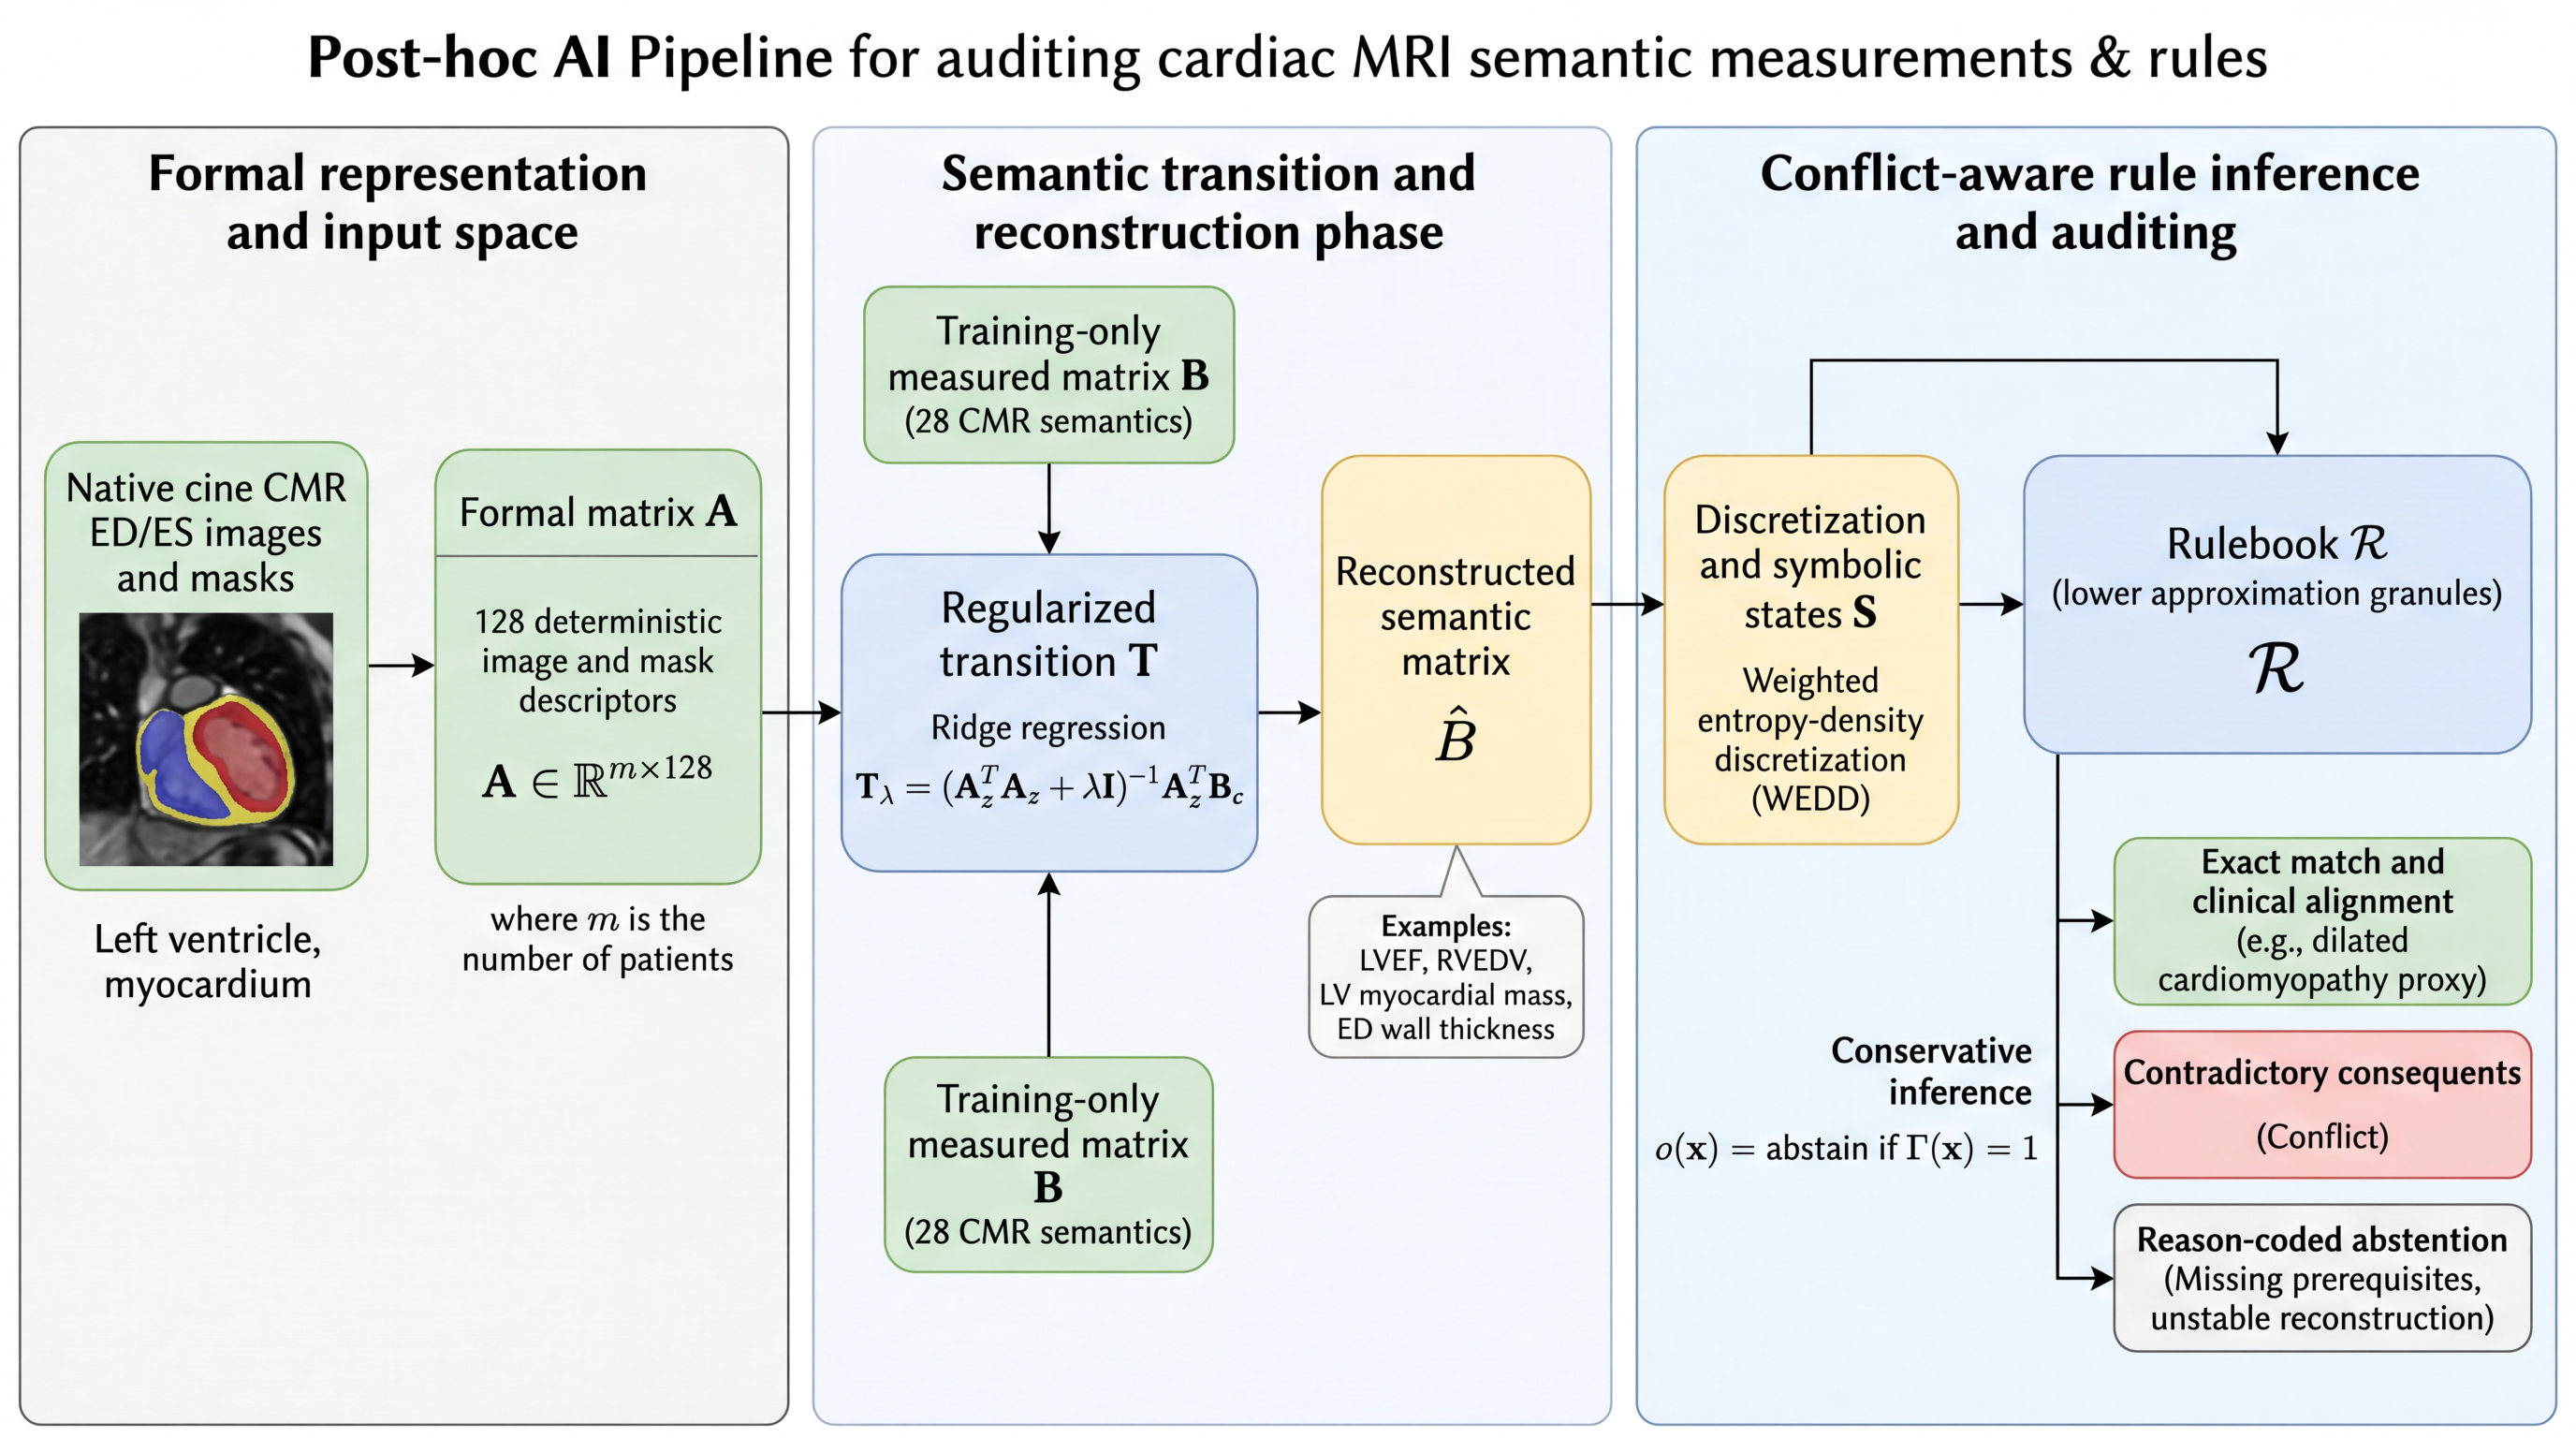
\includegraphics[width=.98\linewidth]{fig_audit-architecture.pdf}
\caption{Post-hoc CMR audit architecture. Training-only measured semantics supervise the transition; held-out inference exposes reconstructed semantics, rule provenance, conflict, and abstention without refitting.}
\label{fig:cmr_audit_architecture}
\end{figure}

The measured semantic matrix \(\matB\in\R^{m\times28}\) contains LV/RV end-diastolic volume (EDV), end-systolic volume (ESV), stroke volume (SV), ejection fraction (EF), LV myocardial volumes and mass, LV--RV SV discrepancy, ED/ES wall thickness and wall thickening, chamber areas, compactness, eccentricity, and LV long-axis length. Accordingly, left-ventricular ejection fraction (LVEF), right-ventricular ejection fraction (RVEF), left-ventricular end-diastolic volume (LVEDV), and right-ventricular end-diastolic volume (RVEDV) denote the corresponding chamber-specific measures used below. The transition \(\matT\in\R^{128\times28}\) reconstructs \(\hatB\); eligible semantics are discretized into \(\matS\), and the rulebook \(\Rule\) returns one auditable consequent or a typed abstention. Transition coefficients are regularized associations, not causal effects or diagnostic criteria.

%% 3.2 Cohorts, patient-disjoint partitions, provenance, and QC gates
\subsection{Datasets, Splits, and Quality Control}\label{subsec:datasets_splits_qc}

ACDC supplied 150 annotated studies in five balanced categories. A fixed patient-disjoint split assigned 85 cases to training, 15 to validation, and 50 to final testing. The external branch contained 100 M\&Ms cases selected once with seed 20260611. Validation, test, and external rows were excluded from every fitted imputation statistic, clipping limit, scaler, regularization choice, transition coefficient, discretization cut, classifier parameter, and rule. Stable \texttt{sample\_id} values linked each matrix row to its source image, mask, metadata, and label. QC checked readability, ED/ES pairing, label domains, voxel spacing, nonempty LV/RV/myocardial masks, plausible volume/EF ranges, finite features, and exact \(\matA\)--\(\matB\) row identity. Feature-level failures blocked only dependent semantics and predicates; high/moderate findings entered manual-review triage with basal, mid-ventricular, and apical overlays. Automated triage identifies cases requiring review but does not constitute expert adjudication. The use of explicit quality prediction is consistent with recent accountable CMR segmentation work~\cite{Gonzales2023QualityControl}.

%% 3.3 Regularized mapping from formal descriptors to CMR semantics
\subsection{Phase 1: Formal-to-Semantic Transition}\label{subsec:formal_to_semantic_transition}

All preprocessing was learned from the 85 training rows: semantic missing values were median-imputed, targets were clipped to their training 1st--99th percentiles, formal columns were standardized, and semantic columns were centered. With standardized \(\matA_z\), centered \(\matB_c\), and ridge penalty \(\lambda\), the transition minimizes the objective in Equation~\eqref{eq:ridge_transition_objective}:
%% Ridge objective for the formal-to-semantic transition.
\begin{equation}
\matT_\lambda=\argmin_{\matT}\left\|\matA_z\matT-\matB_c\right\|_F^2+\lambda\left\|\matT\right\|_F^2 .
\label{eq:ridge_transition_objective}
\end{equation}

The implementation uses the standard closed-form ridge solution in Equation~\eqref{eq:ridge_transition_solution}:
%% Closed-form solution corresponding to the regularized objective.
\begin{equation}
\matT_\lambda=(\matA_z^\top\matA_z+\lambda\mathbf I)^{-1}\matA_z^\top\matB_c .
\label{eq:ridge_transition_solution}
\end{equation}

For a held-out standardized row \(\mathbf a_z\), reconstruction is defined in Equation~\eqref{eq:semantic_reconstruction}:
%% Held-out semantic reconstruction using the frozen transition.
\begin{equation}
\widehat{\mathbf b}(\mathbf a)=\mathbf a_z\matT_\lambda+\boldsymbol\mu_B^\top .
\label{eq:semantic_reconstruction}
\end{equation}

Five-fold stratified cross-validation was restricted to training data and searched \(\lambda\in\{10^{-6},3\times10^{-6},\ldots,30,100\}\); each fold refitted all preprocessing. Candidates were ranked by validation RMSE and then MAE, with solutions within 0.1~\% of the minimum favoring the larger penalty. The selected \(\lambda=3\), feature order, projection checksum, preprocessing state, and \(128\times28\) transition were frozen before validation, test, and external inference.

%% 3.4 Training-only discretization, rule induction, and guarded inference
\subsection{Phase 2: Discretization, Rough Granulation, and Inference}\label{subsec:discretization_granulation_inference}

The current experimental release does not implement the full Weighted Entropy--Density Discretization (WEDD) optimizer. Instead, each eligible semantic feature \(j\) is discretized by training-only tertiles \(q_{j,1/3}\) and \(q_{j,2/3}\), frozen before held-out inference according to Equation~\eqref{eq:tertile_discretization}:
%% Training-only tertile discretization used in the current release.
\begin{equation}
s_j(b)=\begin{cases}
\mathrm{low}, & b\le q_{j,1/3},\\
\mathrm{mid}, & q_{j,1/3}<b\le q_{j,2/3},\\
\mathrm{high}, & b>q_{j,2/3}.
\end{cases}
\label{eq:tertile_discretization}
\end{equation}

This quantile scheme is a documented approximation to the WEDD stage described in the parent framework~\cite{Radiuk2026SEMTRA}; consequently, no result in this paper is claimed to validate full WEDD or to show superiority over alternative discretizers.

The discretized training table is treated as a rough-set decision system~\cite{Pawlak1982Rough}. Cases sharing the same eligible condition states form an indiscernibility granule; a granule enters the lower approximation only when its members share one consequent. Rules have the form shown in Equation~\eqref{eq:production_rule}:
%% Conflict-aware production-rule form induced from rough-set granules.
\begin{equation}
r:\bigwedge_{j\in R_r}[s_j=v_j]\Longrightarrow d=y_r .
\label{eq:production_rule}
\end{equation}

The release retains at most three antecedents, support of at least three training cases, and confidence of at least 0.60. Exact compatible rules fire at inference. If severe QC, unstable reconstruction, a missing prerequisite, no match, or contradictory consequents are present, the output follows Equation~\eqref{eq:guarded_abstention_policy}:
%% Guarded inference policy with explicit reason-coded abstention.
\begin{equation}
o(x)=\begin{cases}
\operatorname{abstain}[\rho(x)], & \Gamma(x)=1,\\
y, & \Gamma(x)=0\ \text{and}\ \mathcal{Y}(x)=\{y\},
\end{cases}
\label{eq:guarded_abstention_policy}
\end{equation}

where \(\rho(x)\) records the reason. Soft similarity never overrides this guard.

%% 3.5 Clinical predicate proxies and rule-alignment similarity
\subsection{Physician-Style Predicates and Similarity}\label{subsec:physician_predicates_similarity}

The predicate library represents cine-supported proxies for dilated and hypertrophic cardiomyopathy, abnormal RV or arrhythmogenic right ventricular cardiomyopathy (ARVC)-like morphology/function, myocardial-infarction remodeling, conservative normality, and review triggers. Tissue characterization, noncompaction, inflammatory or infiltrative disease, flow-dependent valvular disease, and complex congenital anatomy remain unsupported when required sequences or measurements are absent. For physician predicate \(P_y\) and eligible rule \(R_i\), similarity is defined in Equation~\eqref{eq:predicate_rule_similarity}:
%% Similarity between physician-style predicates and eligible rules.
\begin{equation}
\operatorname{Sim}(P_y,R_i)=\max\!\left\{0,
\frac{\sum_jw_j\phi_j(P_y,R_i)}{\sum_jw_j}
-\gamma_cC_i-\gamma_mM_i-\gamma_uU_i+\gamma_aA_i\right\},
\label{eq:predicate_rule_similarity}
\end{equation}

where \(\phi_j\in[0,1]\) is feature compatibility, \(w_j\) is clinical weight, and \(C_i,M_i,U_i,A_i\) encode conflict, missing evidence, instability, and safe abstention.

The best match is the maximum-similarity rule satisfying support, confidence, prerequisite, and validity gates; no missing prerequisite can be compensated by a high similarity score.

%% 3.6 Reconstruction, calibration, selective-rule, and robustness metrics
\subsection{Outcomes and Statistical Protocol}\label{subsec:outcomes_statistical_protocol}

Mean absolute error (MAE) and root-mean-square error (RMSE) use standard definitions~\cite{Willmott2005Advantages}; Pearson correlation follows the conventional product-moment definition~\cite{Benesty2009Pearson}. To compare targets measured in mL, percentage points, mm, g, and dimensionless units, RMSE was normalized by the ACDC-training standard deviation \(s_{j,\mathrm{tr}}\), as defined in Equation~\eqref{eq:sd_nrmse}:
%% Training-SD-normalized reconstruction error used across targets.
\begin{equation}
\operatorname{NRMSE}_j=\operatorname{RMSE}_j/s_{j,\mathrm{tr}} .
\label{eq:sd_nrmse}
\end{equation}

Equation~\eqref{eq:sd_nrmse} is used only for across-target aggregation; mixed-unit MAE/RMSE means are descriptive. Feature-level reporting included Pearson/Spearman correlations, signed bias, Bland--Altman limits, 1,000-resample bias-corrected and accelerated (BCa) 95~\% confidence intervals (CIs) for MAE, and Benjamini--Hochberg false-discovery-rate control at 0.05.

A median-imputed, standardized multinomial logistic regression trained on measured \(\matB\) served as a transparent comparator. Expected calibration error (ECE) used ten equal-mass confidence bins as in Guo et al.~\cite{Guo2017Calibration}. Rule evaluation reported coverage (at least one fired consequent), typed-abstention rate, conflict among covered cases, and balanced accuracy plus macro-F1 on non-abstained cases; coverage and abstention were always reported with selective accuracy to avoid inflated interpretation. Fixed seeds governed partitioning, external-case selection, projection, bootstrapping, and perturbation sampling.

For perturbation \(\tau\) on the fixed 12-case set \(Q\), the relative formal-space change is defined in Equation~\eqref{eq:formal_perturbation_change}:
%% Relative formal-space drift under a fixed perturbation.
\begin{equation}
\Delta_A(\tau)=\frac{1}{|Q|}\sum_{x\in Q}\frac{\|\mathbf a(\tau x)-\mathbf a(x)\|_2}{\|\mathbf a(x)\|_2+\varepsilon}.
\label{eq:formal_perturbation_change}
\end{equation}

Equation~\eqref{eq:formal_perturbation_change} normalizes descriptor drift by the unperturbed formal-vector magnitude for each case. The corresponding mean absolute semantic change across the 28 reconstructed targets is defined in Equation~\eqref{eq:semantic_perturbation_change}:
%% Mean absolute reconstructed-semantic drift under a fixed perturbation.
\begin{equation}
\Delta_B(\tau)=\frac{1}{28|Q|}\sum_{x\in Q}\|\widehat{\mathbf b}(\tau x)-\widehat{\mathbf b}(x)\|_1 .
\label{eq:semantic_perturbation_change}
\end{equation}

Equation~\eqref{eq:semantic_perturbation_change} measures aggregate semantic drift after the frozen transition. The exploratory transformations were 5~\% intensity scaling, one-pixel translations on each in-plane axis, and a \(2^\circ\) rotation. Because \(\Delta_B\) in Equation~\eqref{eq:semantic_perturbation_change} mixes units, it ranks sensitivity only. The reported release deliberately leaves images in their dataset-native orientation; based on the perturbation test, prospective implementations should canonicalize image orientation from spatial metadata before descriptor extraction and, when learned encoders are used, evaluate small-angle rotational augmentation on training data only.

Overall, Algorithm~\ref{alg:cmr_audit_pipeline} specifies the semantic-transition and conflict-aware CMR audit pipeline.

\begin{algorithm}[!htbp]
\caption{Semantic-transition and conflict-aware CMR audit pipeline}
\label{alg:cmr_audit_pipeline}

\textit{Input:} Patient-disjoint ACDC training/validation/test partitions; 
external M\&Ms cohort; paired ED/ES cine images, masks, metadata, and labels.\par

\textit{Output:} Frozen transition \(\matT_\lambda\), reconstructed semantics 
\(\hatB\), symbolic states \(\matS\), rulebook \(\Rule\), audit reports, 
and reason-coded outputs \(o(x)\).

\begin{enumerate}[leftmargin=*,itemsep=2pt,topsep=2pt]

    \item \textbf{Validate and lock cohorts.}
    Verify data integrity, patient independence, QC conditions, and 
    \(\matA\)--\(\matB\) row alignment; then freeze all held-out cohorts.

    \item \textbf{Fit the semantic transition.}
    Learn preprocessing and \(\lambda\) on training data only, estimate 
    \(\matT_\lambda\) using Equations~\eqref{eq:ridge_transition_objective} 
    and~\eqref{eq:ridge_transition_solution}, and reconstruct held-out 
    semantics using Equation~\eqref{eq:semantic_reconstruction}.

    \item \textbf{Discretize eligible semantics.}
    Map valid semantic features to symbolic states using the frozen 
    training tertiles defined in Equation~\eqref{eq:tertile_discretization}.

    \item \textbf{Induce production rules.}
    Form rough-set granules and retain compact rules satisfying the 
    support and confidence constraints in Equation~\eqref{eq:production_rule}.

    \item \textbf{Perform guarded inference.}
    Fire compatible rules and apply 
    Equation~\eqref{eq:guarded_abstention_policy} to return either a 
    single admissible consequent or a reason-coded abstention.

    \item \textbf{Align clinical predicates.}
    Match supported physician-style predicates to eligible rules using 
    Equation~\eqref{eq:predicate_rule_similarity} and the required 
    evidence checks.

    \item \textbf{Evaluate semantic fidelity.}
    Report feature-wise errors and the normalized error defined in 
    Equation~\eqref{eq:sd_nrmse}, together with correlation, bias, 
    uncertainty, and external-shift evidence.

    \item \textbf{Assess perturbation robustness.}
    Measure formal-space and semantic drift on the fixed perturbation 
    subset using Equations~\eqref{eq:formal_perturbation_change} 
    and~\eqref{eq:semantic_perturbation_change}.

\end{enumerate}
\end{algorithm}

%% ====================================================================
%% 4. RESULTS
%% ====================================================================
%% --------------------------------------------------------------------
%% 4. RESULTS: QC, reconstruction, rules, predicates, robustness, SOTA
%% --------------------------------------------------------------------
\section{Results}\label{sec:results}

Results follow the audit chain: cohort/QC integrity in Section~\ref{subsec:cohort_qc_evidence}, semantic reconstruction in Section~\ref{subsec:semantic_reconstruction_results}, transparent classification and rule behavior in Section~\ref{subsec:classification_symbolic_audit}, predicate alignment in Section~\ref{subsec:predicate_alignment_results}, perturbation sensitivity in Section~\ref{subsec:perturbation_diagnostics}, and comparison with published ACDC systems in Section~\ref{subsec:acdc_sota_comparison}.

%% 4.1 Cohort integrity and release-level quality-control evidence
\subsection{Cohort and QC Evidence}\label{subsec:cohort_qc_evidence}

All 250 records retained stable identifiers and exact \(\matA\)--\(\matB\) order. ACDC contained 85 training cases (56.7~\%), 15 validation cases (10.0~\%), and 50 test cases (33.3~\%); all 100 M\&Ms cases were external only. All 20 programmed semantic-matrix gates passed. The workflow generated 53 ACDC and 65 M\&Ms overlay panels. Manual-review triage contained 92 cases across the combined 250-case cohort; this is unresolved review workload, not 92 confirmed segmentation errors or completed expert validation. Table~\ref{tab:cohort_qc_evidence} summarizes the cohort and release-level QC evidence.

%% Table: cohort composition and release-level QC checks.
\begin{table}[!htbp]
\caption{\textbf{Cohort and release-level QC evidence for experiment \texttt{v5\_native\_image\_dss\_100}. The final two rows explicitly state whether values are per cohort or combined.}}
\label{tab:cohort_qc_evidence}
\centering
\small
\begin{tabularx}{\linewidth}{lrrX}
\toprule
Audit item & ACDC & M\&Ms & Scope / interpretation \\
\midrule
Patient-level cases & 150 & 100 & ACDC: 85/15/50 train/validation/test; M\&Ms: external only. \\
Semantic validation checks & 10/10 & 10/10 & All programmed gates passed. \\
Native overlay panels & 53 & 65 & ED/ES image--mask panels generated. \\
Semantic targets per case & 28 & 28 & Same semantic schema evaluated in each cohort. \\
Pending manual-review cases & -- & -- & 92 total across ACDC + M\&Ms; dataset-specific split was not used. \\
\bottomrule
\end{tabularx}
\end{table}

%% 4.2 Internal and external semantic-reconstruction fidelity
\subsection{Semantic Reconstruction Across Datasets}\label{subsec:semantic_reconstruction_results}

Across 28 targets, mean training-SD-normalized RMSE was \(0.510\pm0.148\) in training, \(0.814\pm0.409\) in validation, \(0.767\pm0.246\) on held-out ACDC, and \(1.726\pm1.177\) on external M\&Ms. Table~\ref{tab:transition_aggregate_errors} summarizes these unit-normalized aggregate errors. External NRMSE was 2.25 times the ACDC-test value, demonstrating substantial domain shift.

%% Table: aggregate transition reconstruction across all semantic targets.
\begin{table}[!htbp]
\caption{\textbf{Aggregate transition reconstruction over 28 targets. RMSE and MAE means combine units and are descriptive only.}}
\label{tab:transition_aggregate_errors}
\centering
\small
\begin{tabular}{llrrr}
\toprule
Dataset & Split & SD-NRMSE & RMSE mean & MAE mean \\
\midrule
ACDC & train & \(0.510\pm0.148\) & 33.18 & 26.49 \\
ACDC & validation & \(0.814\pm0.409\) & 58.42 & 46.49 \\
ACDC & test & \(0.767\pm0.246\) & 51.65 & 38.64 \\
M\&Ms & external & \(1.726\pm1.177\) & 85.35 & 69.81 \\
\bottomrule
\end{tabular}
\end{table}

Figure~\ref{fig:transition_split_errors} shows the descriptive mixed-unit MAE/RMSE means; only NRMSE supports across-target comparisons.

%% Figure: split-wise transition reconstruction error.
\begin{figure}[!htbp]
\centering
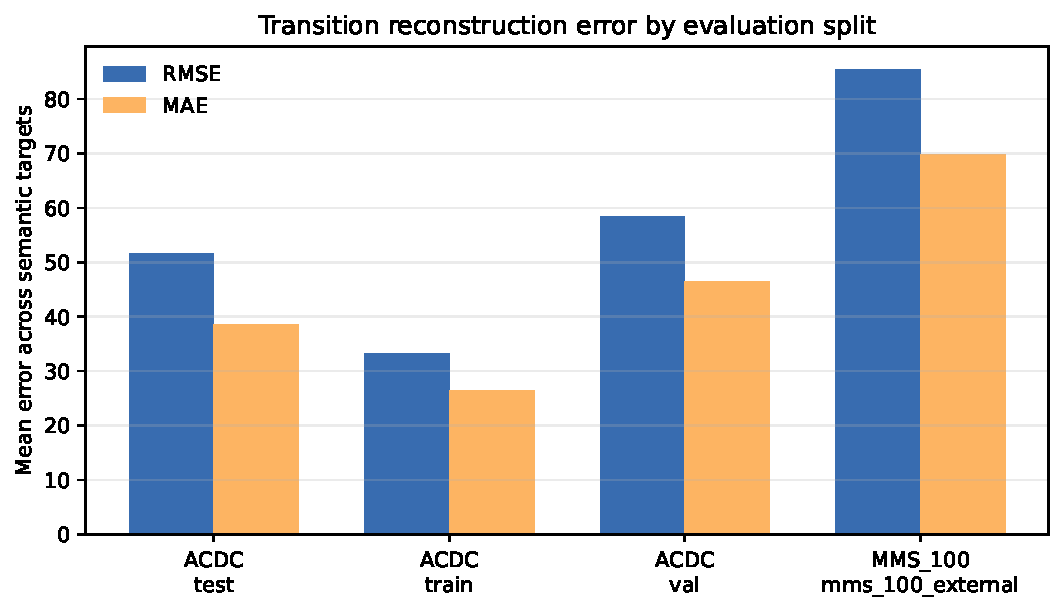
\includegraphics[width=.76\linewidth]{fig_transition_split_errors.pdf}
\caption{Transition reconstruction error by split. Bars are descriptive mixed-unit means.}
\label{fig:transition_split_errors}
\end{figure}

Held-out ACDC fidelity was strongly target-dependent. Global ED wall thickness had \(r=0.928\), LVEF 0.863, RVEF 0.815, RVEDV 0.766, and LVEDV 0.710, whereas LV myocardial mass was 0.517. Table~\ref{tab:high_impact_transition_results} reports the corresponding feature-level errors, correlations, and uncertainty.

%% Table: feature-level held-out ACDC transition fidelity.
\begin{table}[!htbp]
\caption{\textbf{Held-out ACDC transition results (\(n=50\)); intervals are 1,000-resample BCa 95~\% CIs for MAE.}}
\label{tab:high_impact_transition_results}
\centering
\footnotesize
\begin{tabularx}{\linewidth}{Xrrrl}
\toprule
Target & RMSE & MAE (95~\% CI) & Pearson \(r\) & Bias \\
\midrule
Global ED wall thickness (mm) & 0.83 & 0.59 (0.46--0.79) & 0.928 & -0.11 \\
LVEF (percentage points) & 11.38 & 9.17 (7.52--11.16) & 0.863 & -1.93 \\
RVEF (percentage points) & 8.87 & 7.52 (6.33--8.91) & 0.815 & 3.56 \\
LVEDV (mL) & 5.86 & 4.88 (4.02--5.75) & 0.710 & -2.12 \\
RVEDV (mL) & 9.75 & 6.37 (4.89--9.19) & 0.766 & -3.13 \\
LV myocardial mass ED (g) & 4.60 & 3.83 (3.17--4.58) & 0.517 & -1.46 \\
\bottomrule
\end{tabularx}
\end{table}

Figure~\ref{fig:high_impact_correlations} visualizes the high-impact correlations. LVEF MAE was 9.17 percentage points despite high correlation, so threshold-near rule antecedents require guarding. LVEDV had MAE 4.88~mL and bias \(-2.12\)~mL, illustrating that low mean bias does not guarantee patient-level fidelity.

%% Figure: correlations for high-impact reconstructed semantic targets.
\begin{figure}[!htbp]
\centering
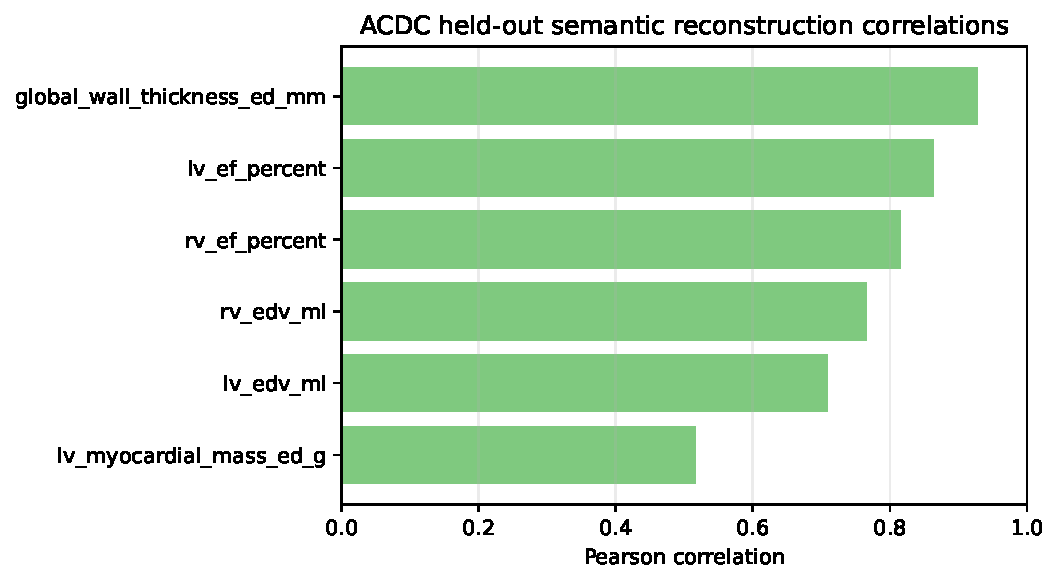
\includegraphics[width=.76\linewidth]{fig_high_impact_correlations.pdf}
\caption{Held-out ACDC Pearson correlations for clinically high-impact semantic targets.}
\label{fig:high_impact_correlations}
\end{figure}

External failure was concentrated in scale-sensitive targets. M\&Ms wall thickness remained comparatively stable (\(r=0.816\), RMSE 0.99~mm), whereas LVEF and RVEF correlations fell to 0.670 and 0.584. LVEDV bias changed from \(-2.12\) to \(-136.0\)~mL and myocardial-mass bias from \(-1.46\) to \(-96.6\)~g. These targets therefore require external recalibration or exclusion before rule inference.

%% 4.3 Transparent semantic classifier and selective rulebook audit
\subsection{Transparent Classification and Symbolic Audit}\label{subsec:classification_symbolic_audit}

The measured-semantic comparator classified 43 of 50 held-out ACDC cases correctly (accuracy and balanced accuracy 0.860), with macro-F1 0.861 and one-vs-rest macro area under the receiver operating characteristic curve (AUROC) 0.973. Table~\ref{tab:semantic_classifier_performance} reports the comparator metrics and row-bootstrap uncertainty. The 95~\% CIs were 0.76--0.94 for accuracy, 0.75--0.95 for balanced accuracy, 0.75--0.94 for macro-F1, and 0.947--0.993 for AUROC. ECE increased from 0.103 in validation to 0.179 on test data.

%% Table: measured-semantic classifier performance and calibration.
\begin{table}[!htbp]
\caption{\textbf{Transparent classifier performance on measured ACDC semantics. ECE uses ten equal-mass bins.}}
\label{tab:semantic_classifier_performance}
\centering
\small
\begin{tabular}{lrrrrrr}
\toprule
Split & Accuracy & Bal. acc. & Macro-F1 & AUROC & ECE & \(n\) \\
\midrule
Validation & 0.933 & 0.933 & 0.931 & 1.000 & 0.103 & 15 \\
Test & 0.860 & 0.860 & 0.861 & 0.973 & 0.179 & 50 \\
\bottomrule
\end{tabular}
\end{table}

The 200-rule layer covered 32 of 50 test cases (0.640) and abstained on 18 (0.360). On non-abstained cases, balanced accuracy was 0.644 and macro-F1 0.612; covered-case conflict was 0.313, and 0.560 of all test cases encountered at least one conflicting rule during resolution. Table~\ref{tab:rulebook_performance} reports the selective rulebook metrics.

%% Table: selective rulebook coverage, abstention, and conflict metrics.
\begin{table}[!htbp]
\caption{\textbf{Rulebook performance. Balanced accuracy and macro-F1 are computed over non-abstained cases.}}
\label{tab:rulebook_performance}
\centering
\footnotesize
\begin{tabular}{lrrrrrrr}
\toprule
Split & Coverage & Abstain & Bal. acc. & Macro-F1 & Conflict & Conf. seen & \(n\) \\
\midrule
Train & 0.565 & 0.435 & 1.000 & 1.000 & 0.229 & 0.565 & 85 \\
Validation & 0.667 & 0.333 & 1.000 & 1.000 & 0.300 & 0.533 & 15 \\
Test & 0.640 & 0.360 & 0.644 & 0.612 & 0.313 & 0.560 & 50 \\
\bottomrule
\end{tabular}
\end{table}

Figure~\ref{fig:classifier_rulebook_outcomes} contrasts the semantic comparator with rulebook outcomes.

%% Figure: comparison of transparent-classifier and rulebook outcomes.
\begin{figure}[!htbp]
\centering
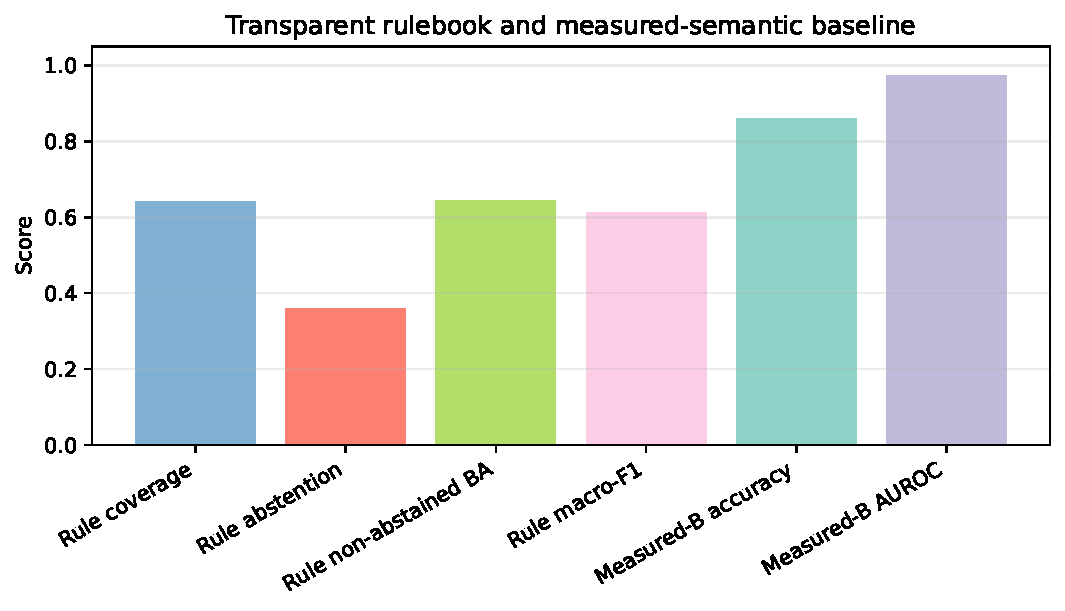
\includegraphics[width=.76\linewidth]{fig_rulebook_classifier_scores.pdf}
\caption{Held-out classifier and rulebook outcomes. Coverage and abstention accompany rule accuracy to prevent selective-performance inflation.}
\label{fig:classifier_rulebook_outcomes}
\end{figure}

These values materially limit practical utility: the rulebook is not a standalone classifier and is not suitable for clinical deployment. Its present value is selective auditability---showing exactly where sparse antecedents agree, conflict, or fail to support a decision. The perfect training/validation non-abstained scores therefore reflect selective, over-specific granules rather than reliable generalization.

%% 4.4 Physician-style predicate alignment and unsupported evidence
\subsection{Predicate Alignment and Unsupported Evidence}\label{subsec:predicate_alignment_results}

The strongest admissible similarity was 0.9008 for abnormal RV/ARVC-like morphology or function, followed by hypertrophic cardiomyopathy (0.8564), myocardial-infarction remodeling (0.8250), and dilated cardiomyopathy (0.7858). Table~\ref{tab:predicate_evidence_alignment} reports the admissible predicate evidence.

%% Table: admissible physician-style predicate evidence and similarity.
\begin{table}[!htbp]
\caption{\textbf{Physician-predicate alignment and evidence status.}}
\label{tab:predicate_evidence_alignment}
\centering
\footnotesize
\begin{tabularx}{\linewidth}{Xlr}
\toprule
Predicate family & Evidence status & Best similarity \\
\midrule
Abnormal RV/ARVC proxy & cine-mask proxy & 0.9008 \\
Hypertrophic cardiomyopathy proxy & cine-mask proxy & 0.8564 \\
Myocardial-infarction remodeling proxy & cine proxy & 0.8250 \\
Dilated cardiomyopathy proxy & cine-mask proxy & 0.7858 \\
Valvular disease volume review & review proxy & 0.7825 \\
Congenital candidate review & research approximation & 0.6842 \\
Conservative normal-state filter & research filter & 0.5462 \\
Restrictive/noncompaction/inflammatory/infiltrative & unsupported & unmatched \\
\bottomrule
\end{tabularx}
\end{table}

Figure~\ref{fig:predicate_alignment_scores} visualizes the corresponding similarity scores.

%% Figure: maximum admissible predicate-to-rule similarity.
\begin{figure}[!htbp]
\centering
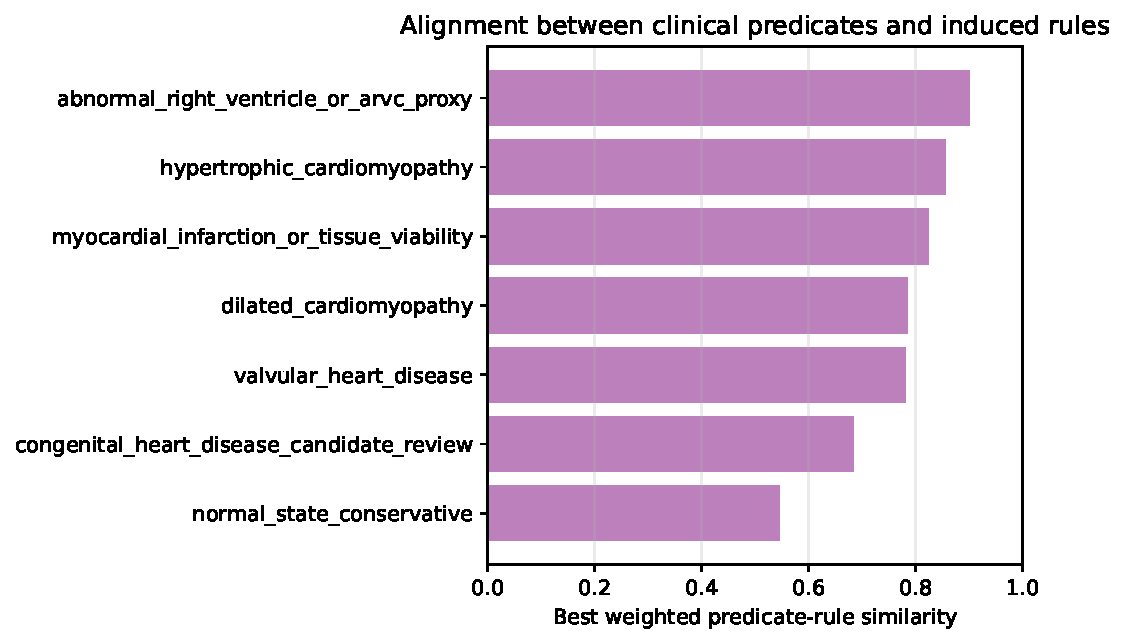
\includegraphics[width=.76\linewidth]{fig_predicate_alignment.pdf}
\caption{Maximum weighted similarity between physician-style predicates and eligible production rules; unsupported predicates are not forced to match.}
\label{fig:predicate_alignment_scores}
\end{figure}

Valvular and congenital proxies remained review-only. Restrictive cardiomyopathy, noncompaction, inflammatory disease, and infiltrative disease were unmatched because cine masks lack the required tissue-characterization evidence; the abstention guard prevented similarity from manufacturing unsupported disease claims.

%% 4.5 Fixed perturbation diagnostics for formal and semantic drift
\subsection{Perturbation Diagnostics}\label{subsec:perturbation_diagnostics}

All 48 case--transformation runs completed. Table~\ref{tab:perturbation_summary} summarizes the four perturbation conditions.

%% Table: fixed perturbation diagnostics on the sampled cases.
\begin{table}[!htbp]
\caption{\textbf{Exploratory perturbation summary over 12 sampled cases; semantic change is a mixed-unit mean.}}
\label{tab:perturbation_summary}
\centering
\small
\begin{tabular}{lrrr}
\toprule
Perturbation & Relative formal change & Semantic change & Mask-count change \\
\midrule
Intensity scale 5~\% & \(1.1\times10^{-8}\) & \(8.8\times10^{-6}\) & 0.000000 \\
Translation x, 1 px & 0.002591 & 0.622935 & 0.000000 \\
Translation y, 1 px & 0.002135 & 0.545662 & 0.000000 \\
Rotation, \(2^\circ\) & 0.053114 & 9.821420 & 0.000470 \\
\bottomrule
\end{tabular}
\end{table}

The 5~\% intensity scaling was numerically negligible, and one-pixel translations produced small formal changes with semantic changes of 0.623 and 0.546. By contrast, a \(2^\circ\) rotation produced relative formal change 0.0531 and mixed-unit semantic change 9.8214, about 20--25 times and 16--18 times the corresponding translation responses. Mask-count change remained 0.000470, indicating orientation sensitivity of the descriptors rather than gross label loss. Because only 12 cases were tested and semantic change mixes units, this is a diagnostic warning rather than a clinical tolerance. The result directly supports canonical orientation normalization before deterministic descriptor extraction and, for future learned encoders, training-only rotational augmentation; neither mitigation is retroactively claimed for the present metrics.

%% 4.6 Task-aware quantitative context against published ACDC systems
\subsection{Quantitative Comparison with ACDC State-of-the-Art Systems}\label{subsec:acdc_sota_comparison}

Table~\ref{tab:acdc_sota_comparison} provides task-aware error and diagnostic-accuracy context rather than a leaderboard claim.

%% Table: task-aware quantitative context against published ACDC systems.
\begin{table}[!htbp]
\caption{\textbf{Task-aware quantitative context on ACDC test cases. MAE units are mL, percentage points, percentage points, and g, respectively. Dashes indicate unreported audit outputs.}}
\label{tab:acdc_sota_comparison}
\centering
\footnotesize
\begin{adjustbox}{max width=\linewidth}
\begin{tabular}{llrrrrrr}
\toprule
System & Source & Diag. acc. & LVEDV MAE & LVEF MAE & RVEF MAE & Mass MAE & Rule cov./BA \\
\midrule
Khened challenge system & \cite{Bernard2018Deep} & 0.960 & 4.20 & 2.50 & 5.30 & 6.30 & --/-- \\
Isensee challenge system & \cite{Bernard2018Deep} & 0.920 & 5.10 & 2.10 & 4.70 & 7.30 & --/-- \\
Proposed transition + semantic baseline & This study & 0.860 & 4.88 & 9.17 & 7.52 & 3.83 & 0.640/0.644 \\
\bottomrule
\end{tabular}
\end{adjustbox}
\end{table}

The proposed diagnostic accuracy was 0.100 below Khened and 0.060 below Isensee. LVEDV MAE (4.88~mL) was comparable to the reported 4.20 and 5.10~mL, but LVEF MAE (9.17 points) was substantially worse than 2.50 and 2.10 points. Mass MAE was lower descriptively, yet the correlation comparison below shows that this did not imply comparable patient-level fidelity.

Table~\ref{tab:acdc_correlation_bias} separately reports correlation, bias, and audit metrics. Bernard et al.~\cite{Bernard2018Deep} evaluated systems that jointly optimized segmentation-derived clinical indices and five-class diagnosis on the official challenge protocol, whereas the present audit uses an independent 85/15/50 split and a deterministic formal representation.

%% Table: ACDC correlation, signed bias, and audit metrics.
\begin{table}[!htbp]
\caption{\textbf{ACDC clinical-index correlation and signed bias. EF bias is in percentage points, LVEDV bias in mL, and mass bias in g. Audit metrics are coverage/abstention/conflict.}}
\label{tab:acdc_correlation_bias}
\centering
%\scriptsize
\begin{adjustbox}{max width=\linewidth}
\begin{tabular}{lccccr}
\toprule
System & LVEF \(r\)/bias & RVEF \(r\)/bias & LVEDV \(r\)/bias & Mass \(r\)/bias & Audit metrics \\
\midrule
Isensee ACDC system & 0.991/+0.5 & 0.925/$-3.0$ & 0.997/+1.5 & 0.986/$-4.0$ & --/--/-- \\
Khened ACDC system & 0.989/$-0.5$ & 0.858/$-2.2$ & 0.997/+0.6 & 0.990/$-2.9$ & --/--/-- \\
Proposed transition and rule audit & 0.863/$-1.93$ & 0.815/+3.56 & 0.710/$-2.12$ & 0.517/$-1.46$ & 0.640/0.360/0.313 \\
\bottomrule
\end{tabular}
\end{adjustbox}
\end{table}

The audit transition trailed the published systems in all four listed correlations; in particular, mass correlation was 0.517 versus 0.986--0.990 despite smaller mean bias. Different splits and objectives preclude a controlled ranking. The contribution is therefore complementary: explicit semantic reconstruction, external-failure evidence, conflict, abstention, and rule provenance rather than diagnostic superiority.

%% ===================================================================
%% SECTION 5: DISCUSSION
%% ===================================================================
%% --------------------------------------------------------------------
%% 5. DISCUSSION: interpretation, limitations, and validation priorities
%% --------------------------------------------------------------------
\section{Discussion}\label{sec:discussion}

The study demonstrates an auditable chain from native CMR images and masks to deterministic formal descriptors, reconstructed measurements, symbolic conditions, and selective rule outputs. This chain should not be conflated with an evaluation of deep latent representations: the current formal space is handcrafted and deterministic. The transition is intentionally linear and inspectable, but its coefficients remain associations rather than causal physiological effects. This restraint is consistent with clinical XAI evidence showing that visually plausible attribution maps can fail requirements for truthfully representing model decision processes and decision quality~\cite{Jin2022MultimodalXAI}.

Three limitations of this study should be highlighted. First, semantic fidelity is target- and domain-dependent, with substantial deterioration on external M\&Ms data; scale-sensitive volume and mass targets require recalibration or exclusion before external rule use. Second, the reported discretizer is a training-quantile approximation, not the complete WEDD optimizer, so full WEDD requires a direct leakage-controlled ablation against quantiles and alternative discretizers. Third, the rule layer's 0.640 coverage and 0.644 non-abstained balanced accuracy materially limit practical utility. The rulebook should therefore be interpreted only as a selective audit artifact that exposes supported, conflicting, and unsupported evidence; it is neither a diagnostic classifier nor a clinically validated decision-support system.

The perturbation experiment identifies a specific engineering weakness rather than a generic robustness claim. A \(2^\circ\) rotation caused the largest change while mask counts were nearly preserved, implicating orientation-sensitive descriptors. Prospective revisions should canonicalize orientation from image spatial metadata before deterministic extraction and evaluate small-angle rotational augmentation when a learned encoder is trained. The current results were not recomputed after such a change, avoiding a post-hoc claim unsupported by the reported experiment. Manual-review triage is also incomplete, and cine-only data cannot support tissue, flow, or complex congenital conclusions.

The next validation stage should attach the same audit layer to frozen high-performing CMR encoders on common patient splits, compare full WEDD with the current quantile approximation, perform vendor-aware recalibration, complete expert QC adjudication, and prospectively test whether provenance, conflict, and abstention improve clinician decisions. These steps align the work with evidence that clinicians prioritize contextual clinical plausibility in XAI and with early-stage clinical-AI evaluation principles.

%% ===================================================================
%% SECTION 6: CONCLUSIONS
%% ===================================================================
%% --------------------------------------------------------------------
%% 6. CONCLUSIONS: evidence boundary and prospective work
%% --------------------------------------------------------------------
\section{Conclusions}\label{sec:conclusions}

This study evaluated a transition-matrix and conflict-aware rule layer on 150 ACDC and 100 external M\&Ms cases. The reported formal representation is a deterministic image--mask descriptor baseline rather than a trained deep encoder, and the discretization stage uses frozen training tertiles rather than full WEDD. On held-out ACDC, mean SD-NRMSE was \(0.767\pm0.246\); LVEF, RVEF, and LVEDV correlations were 0.863, 0.815, and 0.710. The measured-semantic comparator achieved 0.860 accuracy and 0.861 macro-F1. The 200-rule layer provided 0.640 coverage, 0.360 abstention, 0.313 conflict, and 0.644 non-abstained balanced accuracy, which restricts its present role to selective auditing. External SD-NRMSE increased 2.25-fold to \(1.726\pm1.177\), and the rotation diagnostic exposed orientation sensitivity. Accordingly, the current evidence supports transparent failure-aware auditing, not autonomous diagnosis or completed clinical validation.

Future work should evaluate frozen deep encoders on common splits, implement and ablate full WEDD, canonicalize orientation and test rotation-aware training, perform vendor-aware recalibration, complete expert adjudication, and assess the audit outputs prospectively with clinicians.

%% ====================================================================
%% DECLARATIONS
%% ====================================================================
%% --------------------------------------------------------------------
%% DECLARATION ON GENERATIVE AI: CEUR-WS disclosure statement
%% --------------------------------------------------------------------
\section*{Declaration on Generative AI}
During the preparation of this work, the authors utilized generative AI tools to enhance the linguistic quality of this manuscript. The language model Gemini 3.1 Pro Preview (Google LLC) and the language service Grammarly (Grammarly, Inc.) were employed for copyediting assistance, specifically to refine grammar, spelling, and stylistic consistency. Following this, the authors conducted a comprehensive review and revision, ensuring all content accurately reflects their research and conclusions. The authors retain full responsibility for the scientific integrity and final content of this paper.

%% ====================================================================
%% REFERENCES
%% ====================================================================
\bibliography{references}

\end{document}
